\documentclass[twoside]{book}

% Packages required by doxygen
\usepackage{fixltx2e}
\usepackage{calc}
\usepackage{doxygen}
\usepackage[export]{adjustbox} % also loads graphicx
\usepackage{graphicx}
\usepackage[utf8]{inputenc}
\usepackage{makeidx}
\usepackage{multicol}
\usepackage{multirow}
\PassOptionsToPackage{warn}{textcomp}
\usepackage{textcomp}
\usepackage[nointegrals]{wasysym}
\usepackage[table]{xcolor}

% Font selection
\usepackage[T1]{fontenc}
\usepackage[scaled=.90]{helvet}
\usepackage{courier}
\usepackage{amssymb}
\usepackage{sectsty}
\renewcommand{\familydefault}{\sfdefault}
\allsectionsfont{%
  \fontseries{bc}\selectfont%
  \color{darkgray}%
}
\renewcommand{\DoxyLabelFont}{%
  \fontseries{bc}\selectfont%
  \color{darkgray}%
}
\newcommand{\+}{\discretionary{\mbox{\scriptsize$\hookleftarrow$}}{}{}}

% Page & text layout
\usepackage{geometry}
\geometry{%
  a4paper,%
  top=2.5cm,%
  bottom=2.5cm,%
  left=2.5cm,%
  right=2.5cm%
}
\tolerance=750
\hfuzz=15pt
\hbadness=750
\setlength{\emergencystretch}{15pt}
\setlength{\parindent}{0cm}
\setlength{\parskip}{3ex plus 2ex minus 2ex}
\makeatletter
\renewcommand{\paragraph}{%
  \@startsection{paragraph}{4}{0ex}{-1.0ex}{1.0ex}{%
    \normalfont\normalsize\bfseries\SS@parafont%
  }%
}
\renewcommand{\subparagraph}{%
  \@startsection{subparagraph}{5}{0ex}{-1.0ex}{1.0ex}{%
    \normalfont\normalsize\bfseries\SS@subparafont%
  }%
}
\makeatother

% Headers & footers
\usepackage{fancyhdr}
\pagestyle{fancyplain}
\fancyhead[LE]{\fancyplain{}{\bfseries\thepage}}
\fancyhead[CE]{\fancyplain{}{}}
\fancyhead[RE]{\fancyplain{}{\bfseries\leftmark}}
\fancyhead[LO]{\fancyplain{}{\bfseries\rightmark}}
\fancyhead[CO]{\fancyplain{}{}}
\fancyhead[RO]{\fancyplain{}{\bfseries\thepage}}
\fancyfoot[LE]{\fancyplain{}{}}
\fancyfoot[CE]{\fancyplain{}{}}
\fancyfoot[RE]{\fancyplain{}{\bfseries\scriptsize Generated by Doxygen }}
\fancyfoot[LO]{\fancyplain{}{\bfseries\scriptsize Generated by Doxygen }}
\fancyfoot[CO]{\fancyplain{}{}}
\fancyfoot[RO]{\fancyplain{}{}}
\renewcommand{\footrulewidth}{0.4pt}
\renewcommand{\chaptermark}[1]{%
  \markboth{#1}{}%
}
\renewcommand{\sectionmark}[1]{%
  \markright{\thesection\ #1}%
}

% Indices & bibliography
\usepackage{natbib}
\usepackage[titles]{tocloft}
\setcounter{tocdepth}{3}
\setcounter{secnumdepth}{5}
\makeindex

% Custom commands
\newcommand{\clearemptydoublepage}{%
  \newpage{\pagestyle{empty}\cleardoublepage}%
}

\usepackage{caption}
\captionsetup{labelsep=space,justification=centering,font={bf},singlelinecheck=off,skip=4pt,position=top}

%===== C O N T E N T S =====

\begin{document}

% Titlepage & ToC
\pagenumbering{roman}
\begin{titlepage}
\vspace*{7cm}
\begin{center}%
{\Large T\+C\+C\+\_\+\+Nay\+Bru }\\
\vspace*{1cm}
{\large Generated by Doxygen 1.8.11}\\
\end{center}
\end{titlepage}
\clearemptydoublepage
\tableofcontents
\clearemptydoublepage
\pagenumbering{arabic}

%--- Begin generated contents ---
\chapter{Hierarchical Index}
\section{Class Hierarchy}
This inheritance list is sorted roughly, but not completely, alphabetically\+:\begin{DoxyCompactList}
\item \contentsline{section}{chamado}{\pageref{classchamado}}{}
\item \contentsline{section}{dispositivo}{\pageref{classdispositivo}}{}
\item \contentsline{section}{m\+\_\+raci}{\pageref{classm__raci}}{}
\item \contentsline{section}{pessoa}{\pageref{classpessoa}}{}
\item Q\+Dialog\begin{DoxyCompactList}
\item \contentsline{section}{gerencia\+Chamados}{\pageref{classgerencia_chamados}}{}
\item \contentsline{section}{gerencia\+Dispositivo}{\pageref{classgerencia_dispositivo}}{}
\item \contentsline{section}{gerencia\+Pessoas}{\pageref{classgerencia_pessoas}}{}
\item \contentsline{section}{selecionadisp}{\pageref{classselecionadisp}}{}
\item \contentsline{section}{selecionaequip}{\pageref{classselecionaequip}}{}
\item \contentsline{section}{tipo\+Disp}{\pageref{classtipo_disp}}{}
\end{DoxyCompactList}
\item Q\+Main\+Window\begin{DoxyCompactList}
\item \contentsline{section}{Main\+Window}{\pageref{class_main_window}}{}
\end{DoxyCompactList}
\item Q\+Widget\begin{DoxyCompactList}
\item \contentsline{section}{cadastrochamado}{\pageref{classcadastrochamado}}{}
\item \contentsline{section}{cadastrodispositivo}{\pageref{classcadastrodispositivo}}{}
\item \contentsline{section}{Cadastropessoa}{\pageref{class_cadastropessoa}}{}
\item \contentsline{section}{matriz\+R\+A\+CI}{\pageref{classmatriz_r_a_c_i}}{}
\item \contentsline{section}{novo\+Grupo}{\pageref{classnovo_grupo}}{}
\end{DoxyCompactList}
\item \contentsline{section}{status}{\pageref{classstatus}}{}
\item \contentsline{section}{tipod}{\pageref{classtipod}}{}
\end{DoxyCompactList}

\chapter{Class Index}
\section{Class List}
Here are the classes, structs, unions and interfaces with brief descriptions\+:\begin{DoxyCompactList}
\item\contentsline{section}{{\bf cadastrochamado} }{\pageref{classcadastrochamado}}{}
\item\contentsline{section}{{\bf cadastrodispositivo} }{\pageref{classcadastrodispositivo}}{}
\item\contentsline{section}{{\bf Cadastropessoa} }{\pageref{class_cadastropessoa}}{}
\item\contentsline{section}{{\bf Main\+Window} }{\pageref{class_main_window}}{}
\item\contentsline{section}{{\bf matriz\+R\+A\+CI} }{\pageref{classmatriz_r_a_c_i}}{}
\end{DoxyCompactList}

\chapter{Class Documentation}
\section{cadastrochamado Class Reference}
\label{classcadastrochamado}\index{cadastrochamado@{cadastrochamado}}
Inheritance diagram for cadastrochamado\+:\begin{figure}[H]
\begin{center}
\leavevmode
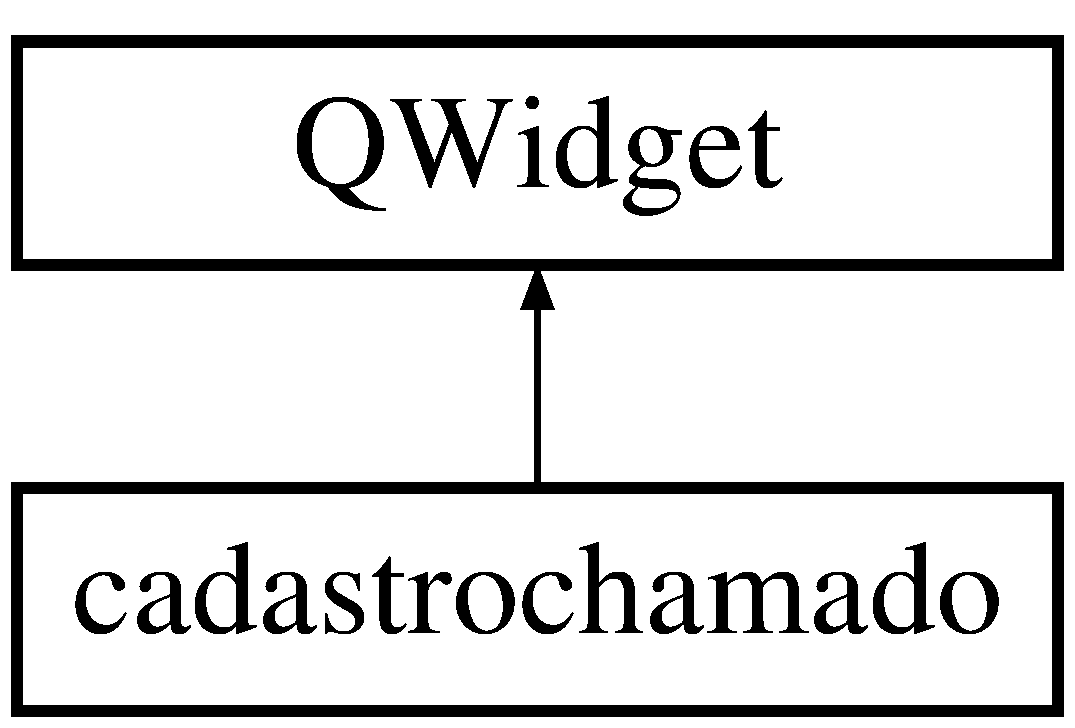
\includegraphics[height=2.000000cm]{classcadastrochamado}
\end{center}
\end{figure}
\subsection*{Public Member Functions}
\begin{DoxyCompactItemize}
\item 
{\bfseries cadastrochamado} (Q\+Widget $\ast$parent=0)\label{classcadastrochamado_a626bec1c5a76c3fe062f70f3fe857c3f}

\end{DoxyCompactItemize}


The documentation for this class was generated from the following files\+:\begin{DoxyCompactItemize}
\item 
D\+:/\+Users/\+Bruno/\+Documents/\+T\+C\+C\+\_\+\+Nay\+Bru/cadastrochamado.\+h\item 
D\+:/\+Users/\+Bruno/\+Documents/\+T\+C\+C\+\_\+\+Nay\+Bru/cadastrochamado.\+cpp\end{DoxyCompactItemize}

\hypertarget{classcadastrodispositivo}{}\section{cadastrodispositivo Class Reference}
\label{classcadastrodispositivo}\index{cadastrodispositivo@{cadastrodispositivo}}


{\ttfamily \#include $<$cadastrodispositivo.\+h$>$}

Inheritance diagram for cadastrodispositivo\+:\begin{figure}[H]
\begin{center}
\leavevmode
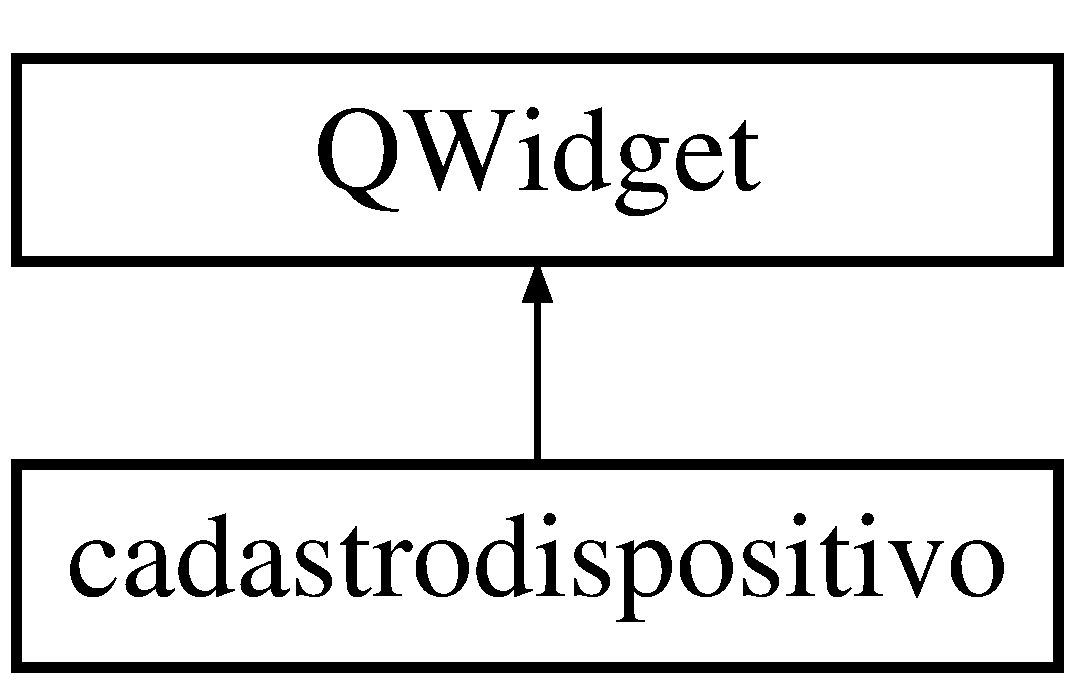
\includegraphics[height=2.000000cm]{classcadastrodispositivo}
\end{center}
\end{figure}
\subsection*{Public Member Functions}
\begin{DoxyCompactItemize}
\item 
\hyperlink{classcadastrodispositivo_a759ec481f21cb002c55d5ca50e8cdf9c}{cadastrodispositivo} (Q\+Widget $\ast$parent=0)
\item 
\hyperlink{classcadastrodispositivo_a21c4cb426f58445706d55dbce57f4aa0}{$\sim$cadastrodispositivo} ()
\end{DoxyCompactItemize}


\subsection{Detailed Description}


Definition at line 10 of file cadastrodispositivo.\+h.



\subsection{Constructor \& Destructor Documentation}
\hypertarget{classcadastrodispositivo_a759ec481f21cb002c55d5ca50e8cdf9c}{}\label{classcadastrodispositivo_a759ec481f21cb002c55d5ca50e8cdf9c} 
\index{cadastrodispositivo@{cadastrodispositivo}!cadastrodispositivo@{cadastrodispositivo}}
\index{cadastrodispositivo@{cadastrodispositivo}!cadastrodispositivo@{cadastrodispositivo}}
\subsubsection{\texorpdfstring{cadastrodispositivo()}{cadastrodispositivo()}}
{\footnotesize\ttfamily cadastrodispositivo\+::cadastrodispositivo (\begin{DoxyParamCaption}\item[{Q\+Widget $\ast$}]{parent = {\ttfamily 0} }\end{DoxyParamCaption})\hspace{0.3cm}{\ttfamily [explicit]}}



Definition at line 5 of file cadastrodispositivo.\+cpp.

\hypertarget{classcadastrodispositivo_a21c4cb426f58445706d55dbce57f4aa0}{}\label{classcadastrodispositivo_a21c4cb426f58445706d55dbce57f4aa0} 
\index{cadastrodispositivo@{cadastrodispositivo}!````~cadastrodispositivo@{$\sim$cadastrodispositivo}}
\index{````~cadastrodispositivo@{$\sim$cadastrodispositivo}!cadastrodispositivo@{cadastrodispositivo}}
\subsubsection{\texorpdfstring{$\sim$cadastrodispositivo()}{~cadastrodispositivo()}}
{\footnotesize\ttfamily cadastrodispositivo\+::$\sim$cadastrodispositivo (\begin{DoxyParamCaption}{ }\end{DoxyParamCaption})}



Definition at line 12 of file cadastrodispositivo.\+cpp.



The documentation for this class was generated from the following files\+:\begin{DoxyCompactItemize}
\item 
C\+:/\+Users/\+Bruno\+S\+R/\+T\+C\+C\+\_\+\+Nay\+Bru/\hyperlink{cadastrodispositivo_8h}{cadastrodispositivo.\+h}\item 
C\+:/\+Users/\+Bruno\+S\+R/\+T\+C\+C\+\_\+\+Nay\+Bru/\hyperlink{cadastrodispositivo_8cpp}{cadastrodispositivo.\+cpp}\end{DoxyCompactItemize}

\hypertarget{class_cadastropessoa}{}\section{Cadastropessoa Class Reference}
\label{class_cadastropessoa}\index{Cadastropessoa@{Cadastropessoa}}


{\ttfamily \#include $<$cadastropessoa.\+h$>$}

Inheritance diagram for Cadastropessoa\+:\begin{figure}[H]
\begin{center}
\leavevmode
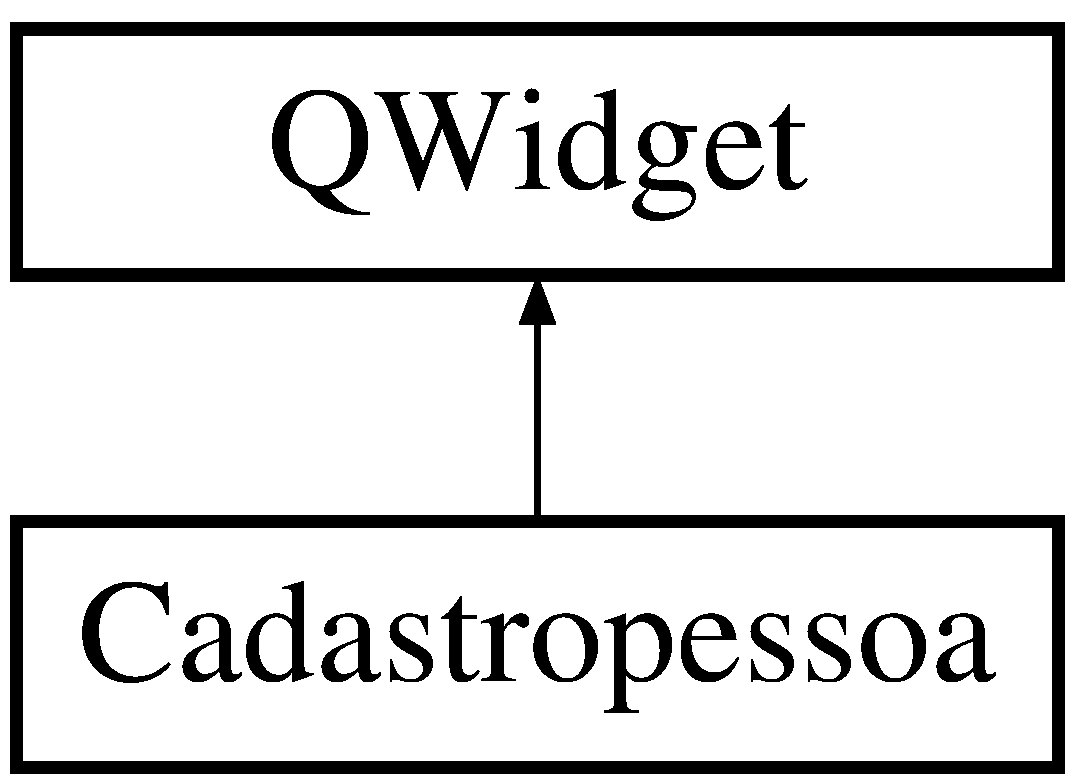
\includegraphics[height=2.000000cm]{class_cadastropessoa}
\end{center}
\end{figure}
\subsection*{Public Member Functions}
\begin{DoxyCompactItemize}
\item 
\hyperlink{class_cadastropessoa_a706230f399727160a6fd25592f77da12}{Cadastropessoa} (Q\+Widget $\ast$parent=0)
\item 
\hyperlink{class_cadastropessoa_a19e6b26d15f77eb6844e67b1246661cf}{$\sim$\+Cadastropessoa} ()
\end{DoxyCompactItemize}


\subsection{Detailed Description}


Definition at line 10 of file cadastropessoa.\+h.



\subsection{Constructor \& Destructor Documentation}
\hypertarget{class_cadastropessoa_a706230f399727160a6fd25592f77da12}{}\label{class_cadastropessoa_a706230f399727160a6fd25592f77da12} 
\index{Cadastropessoa@{Cadastropessoa}!Cadastropessoa@{Cadastropessoa}}
\index{Cadastropessoa@{Cadastropessoa}!Cadastropessoa@{Cadastropessoa}}
\subsubsection{\texorpdfstring{Cadastropessoa()}{Cadastropessoa()}}
{\footnotesize\ttfamily Cadastropessoa\+::\+Cadastropessoa (\begin{DoxyParamCaption}\item[{Q\+Widget $\ast$}]{parent = {\ttfamily 0} }\end{DoxyParamCaption})\hspace{0.3cm}{\ttfamily [explicit]}}



Definition at line 5 of file cadastropessoa.\+cpp.

\hypertarget{class_cadastropessoa_a19e6b26d15f77eb6844e67b1246661cf}{}\label{class_cadastropessoa_a19e6b26d15f77eb6844e67b1246661cf} 
\index{Cadastropessoa@{Cadastropessoa}!````~Cadastropessoa@{$\sim$\+Cadastropessoa}}
\index{````~Cadastropessoa@{$\sim$\+Cadastropessoa}!Cadastropessoa@{Cadastropessoa}}
\subsubsection{\texorpdfstring{$\sim$\+Cadastropessoa()}{~Cadastropessoa()}}
{\footnotesize\ttfamily Cadastropessoa\+::$\sim$\+Cadastropessoa (\begin{DoxyParamCaption}{ }\end{DoxyParamCaption})}



Definition at line 12 of file cadastropessoa.\+cpp.



The documentation for this class was generated from the following files\+:\begin{DoxyCompactItemize}
\item 
C\+:/\+Users/\+Bruno\+S\+R/\+T\+C\+C\+\_\+\+Nay\+Bru/\hyperlink{cadastropessoa_8h}{cadastropessoa.\+h}\item 
C\+:/\+Users/\+Bruno\+S\+R/\+T\+C\+C\+\_\+\+Nay\+Bru/\hyperlink{cadastropessoa_8cpp}{cadastropessoa.\+cpp}\end{DoxyCompactItemize}

\hypertarget{class_main_window}{}\section{Main\+Window Class Reference}
\label{class_main_window}\index{Main\+Window@{Main\+Window}}


{\ttfamily \#include $<$mainwindow.\+h$>$}

Inheritance diagram for Main\+Window\+:\begin{figure}[H]
\begin{center}
\leavevmode
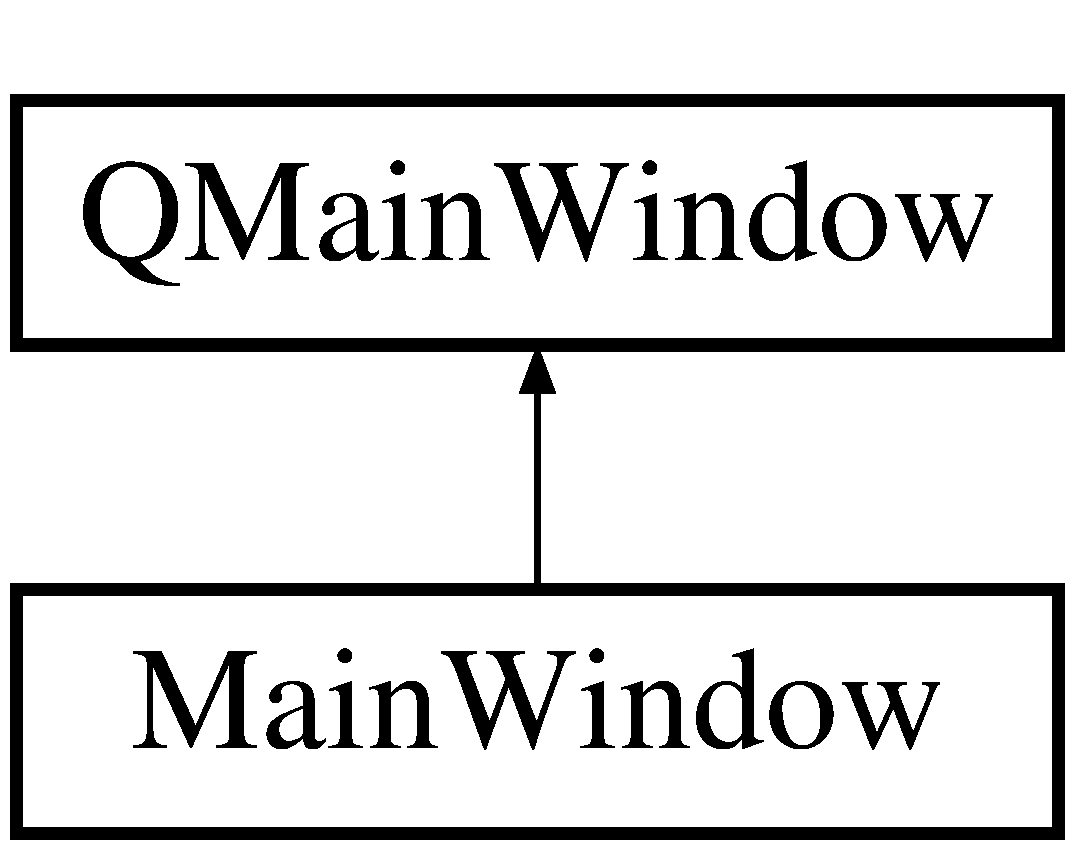
\includegraphics[height=2.000000cm]{class_main_window}
\end{center}
\end{figure}
\subsection*{Public Member Functions}
\begin{DoxyCompactItemize}
\item 
\hyperlink{class_main_window_a8b244be8b7b7db1b08de2a2acb9409db}{Main\+Window} (Q\+Widget $\ast$parent=0)
\item 
\hyperlink{class_main_window_ae98d00a93bc118200eeef9f9bba1dba7}{$\sim$\+Main\+Window} ()
\end{DoxyCompactItemize}


\subsection{Detailed Description}


Definition at line 27 of file mainwindow.\+h.



\subsection{Constructor \& Destructor Documentation}
\hypertarget{class_main_window_a8b244be8b7b7db1b08de2a2acb9409db}{}\label{class_main_window_a8b244be8b7b7db1b08de2a2acb9409db} 
\index{Main\+Window@{Main\+Window}!Main\+Window@{Main\+Window}}
\index{Main\+Window@{Main\+Window}!Main\+Window@{Main\+Window}}
\subsubsection{\texorpdfstring{Main\+Window()}{MainWindow()}}
{\footnotesize\ttfamily Main\+Window\+::\+Main\+Window (\begin{DoxyParamCaption}\item[{Q\+Widget $\ast$}]{parent = {\ttfamily 0} }\end{DoxyParamCaption})\hspace{0.3cm}{\ttfamily [explicit]}}



Definition at line 9 of file mainwindow.\+cpp.

\hypertarget{class_main_window_ae98d00a93bc118200eeef9f9bba1dba7}{}\label{class_main_window_ae98d00a93bc118200eeef9f9bba1dba7} 
\index{Main\+Window@{Main\+Window}!````~Main\+Window@{$\sim$\+Main\+Window}}
\index{````~Main\+Window@{$\sim$\+Main\+Window}!Main\+Window@{Main\+Window}}
\subsubsection{\texorpdfstring{$\sim$\+Main\+Window()}{~MainWindow()}}
{\footnotesize\ttfamily Main\+Window\+::$\sim$\+Main\+Window (\begin{DoxyParamCaption}{ }\end{DoxyParamCaption})}



Definition at line 17 of file mainwindow.\+cpp.



The documentation for this class was generated from the following files\+:\begin{DoxyCompactItemize}
\item 
C\+:/\+Users/\+Bruno\+S\+R/\+T\+C\+C\+\_\+\+Nay\+Bru/\hyperlink{mainwindow_8h}{mainwindow.\+h}\item 
C\+:/\+Users/\+Bruno\+S\+R/\+T\+C\+C\+\_\+\+Nay\+Bru/\hyperlink{mainwindow_8cpp}{mainwindow.\+cpp}\end{DoxyCompactItemize}

\section{matriz\+R\+A\+CI Class Reference}
\label{classmatriz_r_a_c_i}\index{matriz\+R\+A\+CI@{matriz\+R\+A\+CI}}
Inheritance diagram for matriz\+R\+A\+CI\+:\begin{figure}[H]
\begin{center}
\leavevmode
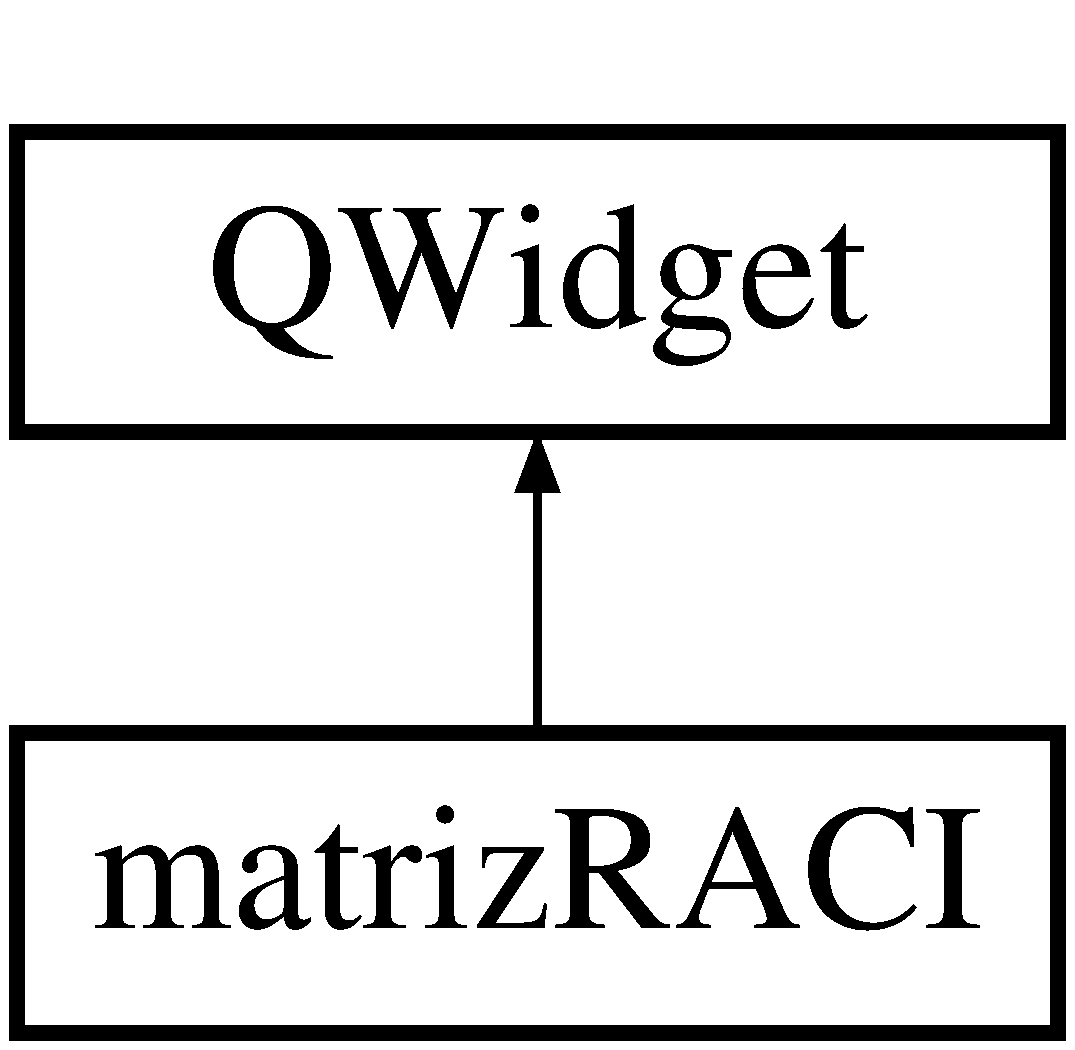
\includegraphics[height=2.000000cm]{classmatriz_r_a_c_i}
\end{center}
\end{figure}
\subsection*{Public Member Functions}
\begin{DoxyCompactItemize}
\item 
{\bfseries matriz\+R\+A\+CI} (Q\+Widget $\ast$parent=0)\label{classmatriz_r_a_c_i_ae380d9647713f9dc8c4dbc275f69a672}

\end{DoxyCompactItemize}


The documentation for this class was generated from the following files\+:\begin{DoxyCompactItemize}
\item 
D\+:/\+Users/\+Bruno/\+Documents/\+T\+C\+C\+\_\+\+Nay\+Bru/matrizraci.\+h\item 
D\+:/\+Users/\+Bruno/\+Documents/\+T\+C\+C\+\_\+\+Nay\+Bru/matrizraci.\+cpp\end{DoxyCompactItemize}

%--- End generated contents ---

% Index
\backmatter
\newpage
\phantomsection
\clearemptydoublepage
\addcontentsline{toc}{chapter}{Index}
\printindex

\end{document}
